% !TeX root = rapport.tex
\section{Presentation}\label{presentation}

The LAMSADE is an historical research unit (established in 1974) originally created around the domain of Management Science and Operational Research, and then having evolved into Computer Science while keeping a very specific identity: Decision Sciences and Technologies. In this long history the unit has kept clear three distinctive features of its identity: \\
 - an original vision of Decision Sciences and Technologies, including an interdisciplinary perspective; \\
 - an international leadership through the establishment and the conduction of ``research communities''; \\
 - a wise blend between foundational and applied research, the field of decision sciences and technologies being specifically characterised by the necessity to keep the frontiers between these two fields widely open.

The research conducted within the LAMSADE aims at approaching the problem of improving both decision making and decision support (aiding to decision making) taking into account the axiomatic, algorithmic and pragmatic dimensions of these topics. The axiomatic dimension includes research on the foundations of decision models, preference models, learning procedures, optimisation techniques, reasoning formalisms, formal languages (from representation ones such as graph theory to query languages for massive data bases). The algorithmic dimension includes research on complexity, parametrised complexity, more generally about the efficiency of structures (data, knowledge etc.), of procedures (optimisation, learning, computing) and services (both computer guided ones such as web services and human guided ones such as health services). The pragmatic dimension includes research both on foundational topics (What is a decision problem? How to formulate a decision problem?) and on practical ones (How to conduct decision aiding activities within a given problem context? How to measure the impact of a policy? How to consider the intervention of decision aiding within a decision process? What is the organisational impact of decision aiding?).

The research questions addressed by the LAMSADE naturally conducted us beyond the frontiers of computer science towards mathematics (optimisation, game theory, statistical learning), economics (social choice theory, game theory, econometrics), social sciences (policy impact, measurement, peace studies), management (theory of innovation, design theory, public management) and more recently law (data protection, data privacy, social responsibility of algorithms). On such subjects the LAMSADE entertains solid relations with all research units of Université Paris-Dauphine (co-tutoring of PhD students, joint seminars, joint training programs, joint research projects) besides including within it a relatively large component of researchers who are not computer scientists.

Since its foundation, the LAMSADE has had a role of international leadership creating and/or helping to conduct international research communities. It has been the case with the creation of the European Working Group on Multiple Criteria Decision Analysis (established in 1975 and since then meeting every 6 months; we will actually organise the 86th meeting in September 2017). It has been also the case with the Algorithmic Decision Theory community (established in 2007,  meeting every two year since then the next conference being scheduled in October 2017 at Luxembourg, and supported by a CNRS GDRI: \url{www.algodec.org}), as well as with the International Symposium on Combinatorial Optimisation, not to mention our implication in communities such as Computational Social Choice or Game Theory. Our last creation has been the Policy Analytics community, nationally supported by a CNRS GDR (\url{www.gdr3720.fr}. This distinctive feature of our research makes the LAMSADE a unique research unit in the domain of the Decision Sciences and Technologies.

The mission of the LAMSADE is essentially to conduct fundamental research in its area of expertise, and we are proud to have been able to do that (despite this not always being the priority of the national and European policy). This being said, the field of Decision Sciences and Technologies requires strong connections with the real world, since it aims at helping real decision makers to improve the ways through which they handle real decision problems. We are equally proud to have been able to maintain such strong connections through a wide network of industrial and policy making partners feeding our research with empirical findings, new challenges and, last but not least, with critical resources otherwise unreachable.

\subsection{History and location of the unit.}\label{history}

As already mentioned, the LAMSADE was established in 1974, and became a joint CNRS/Université Paris-Dauphine research unit in 1976. This institutional configuration remained unchanged in these 42 years. However, it should not conceal the profound evolution of the unit. Focussing on the period under assessment it should be mentioned that the LAMSADE in 2012 was organised in two large teams: ``Decision'' and ``Algorithms/Optimisation/Data''. This structure was completed by a number of ``projects''. This has been the result of a large restructuration which took place during the period 2007-2011 and which has been validated by the previous evaluation exercice (in 2012).

During this last period the LAMSADE decided to re-open the discussion about its internal organisation on the basis of a scientific policy assessment: a research unit dedicated to Decision Sciences and Technologies could not be missing a strong independent team in key areas related to the management and structuring of data, their applications and challenges. For this purpose, starting 2015 we conducted a long internal discussion which resulted to the establishment (starting January 2016) of a third large team named ``Data Sciences''. At the same time a number of projects have been discontinued (namely ``Management of Services'' and ``Knowledge Management''), while a number of new ones have been created. The present structure of the LAMSADE can be seen in \cref{organisation-en}.

%\begin{table}
%  \centering
%   \scalebox{0.85}{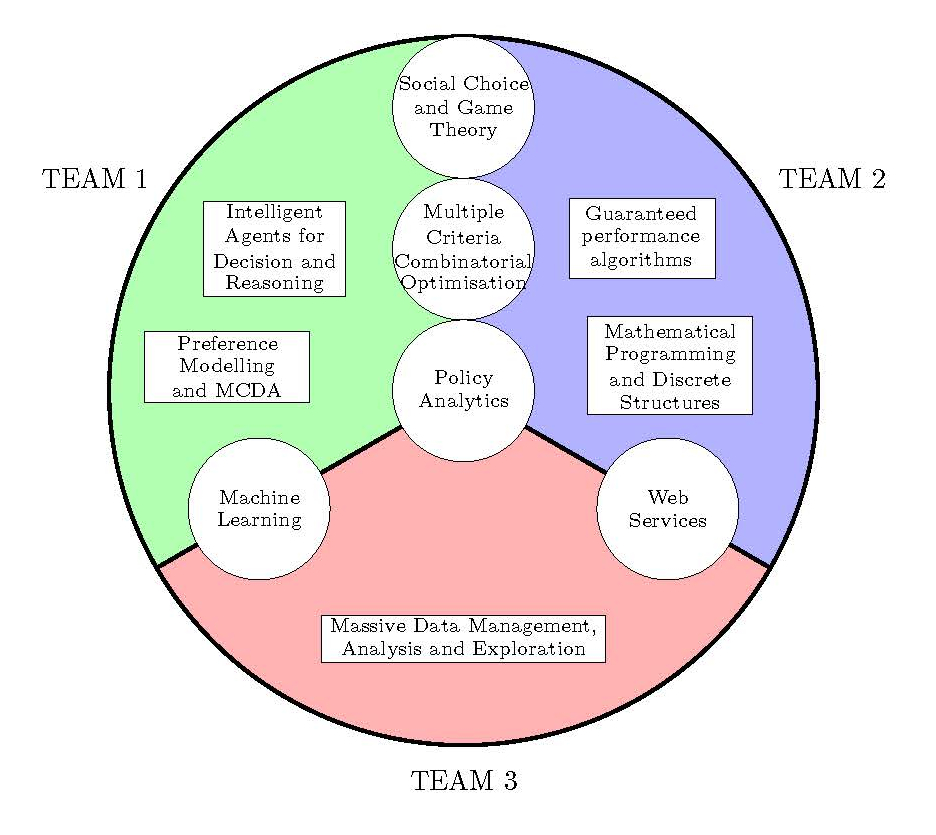
\includegraphics{organisation-en.jpg}}
%  \caption{Organisational chart of the LAMSADE structure}\label{organisation-en}
%\end{table}

\begin{figure}
	\centering
	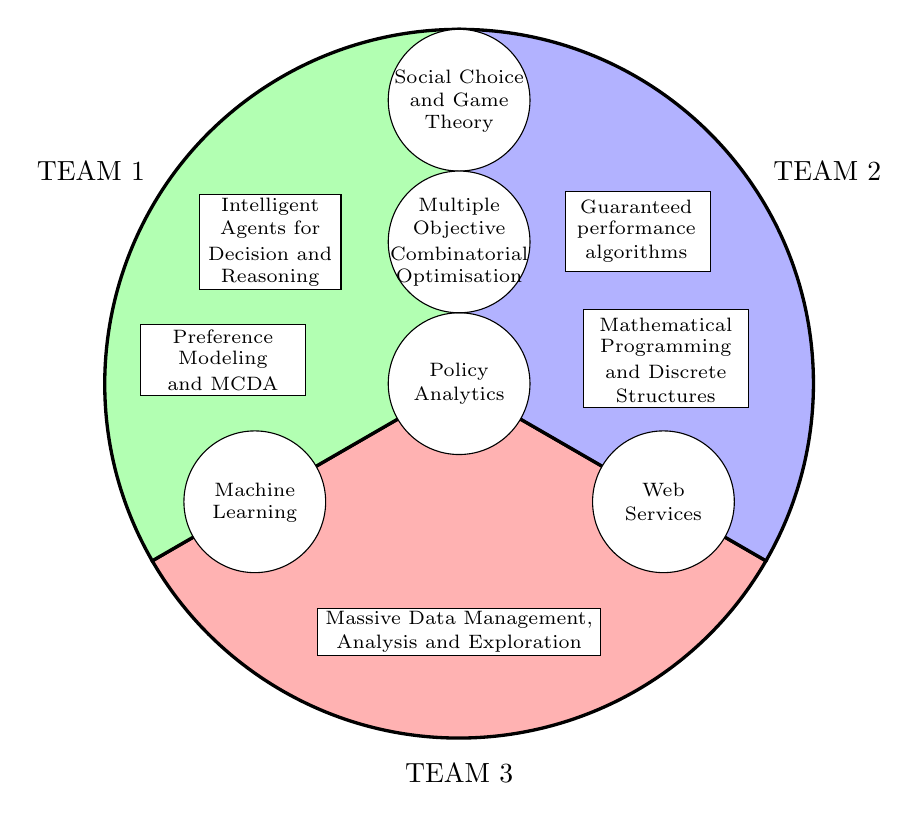
\begin{tikzpicture}[scale=1.5]

%\draw [very thick,black,fill=gray!20](0,0) circle (3) ;

\draw [very thick,fill=red!30](3 * 0.866,3 * -0.5) arc (330:210:3) -- (0,0) -- cycle;
\draw [very thick,fill=green!30](3 * -0.866,3 * -0.5) arc (210:90:3) -- (0,0) -- cycle;
\draw [very thick,fill=blue!30](0,3) arc (90:-30:3) -- (0,0) -- cycle;
%\draw [very thick,fill=gray!45](0,3) arc (90:-30:3) ;


%\draw [thick] (0,0.60) -- (0,1.25) ;
%\draw [thick] (0,3) -- (0,2.75) ;



\draw [thick] (0.60 * -0.866,0.60 * -0.5) -- (1.4 * -0.866,1.4 * -0.5) ;
\draw [thick] (2.6 * -0.866,2.6 * -0.5) -- (3 * -0.866,3 * -0.5) ;


\draw [thick] (0.60 * 0.866,0.60 * -0.5) -- (1.4 * 0.866,1.4 * -0.5) ;
\draw [thick] (2.6 * 0.866,2.6 * -0.5) -- (3 * 0.866,3 * -0.5) ;


\draw [fill=gray!00] (0,0) circle (0.60) ;
\draw (0,0.1) node{{\scriptsize Policy}} ;
\draw (0,-0.1) node{{\scriptsize Analytics}} ;

\draw [fill=gray!00](0,2.4) circle (0.6) ;
\draw (0,2.6) node{{\scriptsize Social Choice}} ;
\draw (0,2.4) node{{\scriptsize and Game }};
\draw (0,2.2) node{{\scriptsize Theory}} ;


\draw [fill=gray!00](0,2.2-1) circle (0.6) ;
\draw (0,2.5-1) node{{\scriptsize Multiple}} ;
\draw (0,2.3-1) node{{\scriptsize Objective}} ;
\draw (0,2.1-1) node{{\scriptsize Combinatorial}};
\draw (0,1.9-1) node{{\scriptsize Optimisation}} ;



%\draw (1.1,1.1) rectangle (1.9,1.9);
%\draw (1.5,1.5) node{{\tiny Programmation }} ;
%\draw (1.5,1.3) node{{\tiny Math\'ematiques}} ;

\draw [fill=gray!00](1.05,-0.2) rectangle (2.45,0.63) ;
\draw (1.75,0.5) node{{\scriptsize Mathematical }} ;
\draw (1.75,0.3) node{{\scriptsize Programming}} ;
\draw (1.75,0.1) node{{\scriptsize and Discrete}} ;
\draw (1.75,-0.1) node{{\scriptsize Structures}} ;


\draw [fill=gray!00](0.9,0.95) rectangle (2.13,1.63) ;
\draw (1.5,1.5) node{{\scriptsize Guaranteed }} ;
\draw (1.5,1.3) node{{\scriptsize performance}} ;
\draw (1.5,1.1) node{{\scriptsize algorithms}} ;


\draw [fill=gray!00](-1.2,-2.3) rectangle (1.2,-1.9) ;
\draw (0,-2.0) node{{\scriptsize Massive Data Management,}} ;
\draw (0,-2.2) node{{\scriptsize Analysis and Exploration}} ;

%\draw (0.9,-2.0) node{{\tiny Services}} ;

\draw [fill=gray!00](-2.7,-0.1) rectangle (-1.3,0.50) ;
\draw (-2.0,0.4) node{{\scriptsize Preference }} ;
\draw (-2.0,0.2) node{{\scriptsize Modeling }} ;
\draw (-2.0,0.0) node{{\scriptsize and MCDA}} ;

%\draw (-1.8,1.0) node{{\tiny Optimisation}} ;
%\draw (-1.8,0.8) node{{\tiny Multicrit\`ere}} ;

\draw [fill=gray!00](-2.2,0.8) rectangle (-1.0,1.6) ;
\draw (-1.6,1.5) node{{\scriptsize Intelligent }} ;
\draw (-1.6,1.3) node{{\scriptsize Agents for }} ;
\draw (-1.6,1.1) node{{\scriptsize Decision and}} ;
\draw (-1.6,0.9) node{{\scriptsize Reasoning}} ;

\draw [fill=gray!00](-1.73,-1) circle (0.6) ;
\draw (-1.73,-1.1) node{{\scriptsize Learning}} ;
\draw (-1.73,-0.9) node{{\scriptsize Machine}} ;

\draw [fill=gray!00](1.73,-1) circle (0.60) ;
\draw (1.73,-0.9) node{{\scriptsize Web}} ;
\draw (1.73,-1.1) node{{\scriptsize Services}} ;

\draw (3.6 * -0.866,3.6 * 0.5) node{TEAM 1} ;
\draw (3.6 * 0.866,3.6 * 0.5) node{TEAM 2} ;
\draw (0,-3.3) node{TEAM 3} ;


\end{tikzpicture}

	\caption{Organisational chart of the LAMSADE structure}\label{organisation-en}
\end{figure}

The three teams of LAMSADE (Decision, Algorithms/Optimisation and Data Sciences) have essentially a mission of scientific animation (seminars, lectures, long term policy etc.) and receive a budget from the general budget of the unit (more details at section \ref{Management}). The research mission of the unit is accomplished by the 10 research projects:
\begin{itemize}
\item Preference Modeling and Multiple Criteria Decision Aiding;
\item Intelligent Agents for Decision and Reasoning;
\item Multiple Objective Combinatorial Optimisation (MOCO);
\item Machine Learning;
\item Massive Data Management, Analysis and Exploration (MADAX);
\item Web Services;
\item Mathematical Programming and Discrete Structures (Mathis);
\item Guaranteed Performance Algorithms (AGaPe);
\item Games and Social Choice: Axiomatic and Computational Aspects;
\item Policy Analytics.
\end{itemize}
These projects are aimed to conduct fundamental and applied research towards long term scientific or societal challenges.

Until recently the unit did not require any specialised computer equipment, the existing servers and network being sufficient. The establishment of the Data Sciences team and the more recent deep learning experiments conducted within the Intelligent Agents project pushed the unit to invest in the creation of a ``Big Data Cluster'' (co-funded by the LAMSADE, the CEREMADE and the MIDO Department, and managed by the LAMSADE) as well as to acquire dedicated hardware for deep learning experiments.

The unit is located at the main campus of Université Paris-Dauphine, and currently occupies 40 offices. However, this hardly covers our needs in individual and collective work space, the most critical situation concerning the PhD students and the post-docs. Equally importantly, these offices are still scattered in the building (two at the 2nd floor, eight at the 4th floor and thirty at the 6th floor), with some obvious negative consequences for the collective life of the unit. Unfortunately, until today the university has been unable to give a long-term satisfactory reply to our demand for a more appropriate location of our activities.

\subsection{Workforce and resources of the unit}\label{workforce}

This section is divided in three parts: the first one concerns the permanent scientific staff as well as the administrative one; the second one concerns the PhD students and the post-docs; the third one concerns the global resources of the LAMSADE.

\begin{table}
  \centering
   \scalebox{0.65}{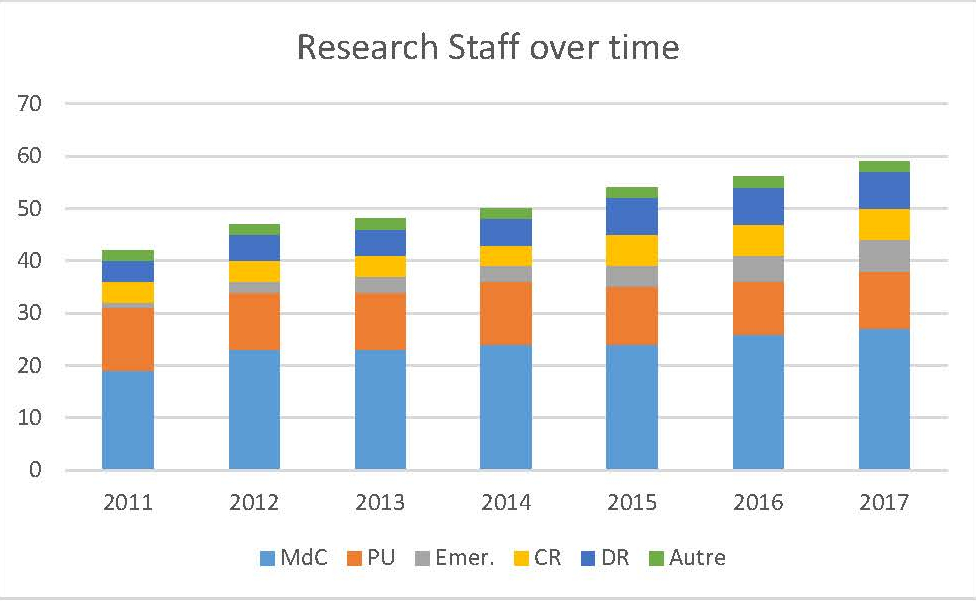
\includegraphics{staffovertime.jpg}}
  \caption{Evolution of research staff since the last report}\label{stafovertime}
\end{table}

Table \ref{stafovertime} presents the evolution of the permanent scientific staff of the unit. However, it does not explain the whole mobility process that has affected the LAMSADE for the last five years. In 2011 (when the last report was presented) the unit had 42 permanent scientific members, divided as follows: 19 associate professors (of which 3 belonging to other universities), 12 full professors (of which 1 belonging to another university), 4 CNRS junior researchers, 4 CNRS research directors, 1 emeritus, and 2 other researchers. At the time the present report is written, the LAMSADE has 56 permanent scientific members: 26 associate professors (among which 3 `externals'), 10 full professors (among which 1 `external'), 6 CNRS junior researchers, 7 CNRS research directors, 5 emeritus and 2 others, and with certainty will have 59 permanent scientific members in 2018 and 60 in 2019. During these 5 years, the LAMSADE presented on average more than 10 candidates annually for CNRS positions. As a result, we have seen the arrival of 3 CNRS research directors and 2 CNRS junior researchers (4 of these new CNRS personnel not being computer scientists). Meanwhile, 4 full professors retired (3 of which have been replaced or will shortly be, and one, in management science, has not been replaced by someone belonging to the LAMSADE), 5 associate professors left (4 of which were promoted to full professors\footnote{Université Pierre et Marie Curie, École de Mines de St. Etienne, École de Mines de Nancy, University of Freiburg in Switzerland}, and one moved to the private sector; all but one have been replaced), 5 more associate professors arrived (due to the retirement of 6 associate professors in computer science who were not members of the LAMSADE, since they did not have a research activity). All recruitements have been `externals' (no local PhD student was hired as associate professor, and no local associate professor was promoted to full professor), and for a large part international\footnote{2 full professors arrived from Université Paris Sud and one is on arrival from Université Paris 13. The 11 Associate professors recruited in this period arrived from post-doc positions: 3 from Japan (Universities of Tokyo and Kyoto), 2 from ILLC in Amsterdam, and 1 from Paris 13, from École Polytechnique, 1 from University of Manchester, 1 from INRIA Nantes, 1 from Université d'Orleans and 1 from University of Luxembourg}. Unfortunately, there has also been a recruitement by the university of a local PhD student, reason for which this colleague, although being a computer scientist, is not a member of the LAMSADE. At present, the unit hosts mosts of the computer scientists of Dauphine (more precisely, all of them but two), plus 6 CNRS scientists who are not computer scientists (essentially economists and management scientists). Summarising: in 5 years the LAMSADE renewed more than one third of its permanent scientific staff, giving at the same time a strong impulse to its scientific innovation and moving its median age towards the 30s (see the age line in table \ref{ageline}). It is important to note that at the beginning of the period under report the LAMSADE had 7 administrative staff working for the equivalent time of 5. Today the unit has 5 administrative staff, all of them occupied 100\% of their time (which thus has remained constant over time). Among these 5, 2 are permanent CNRS staff (one secretary and the computer engineer of the unit), 1 is a permanent employee of Dauphine (a secretary) and two are employees under contract (a secretary and the head of the administrative staff of the LAMSADE).

\begin{table}
  \centering
   \scalebox{0.65}{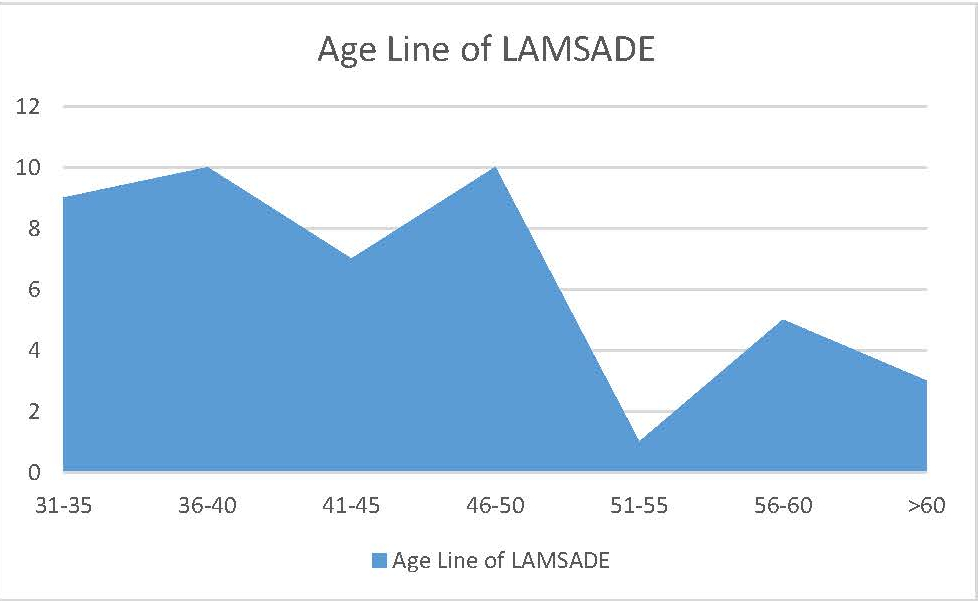
\includegraphics{ageline.jpg}}
  \caption{Age line of the research staff in LAMSADE}\label{ageline}
\end{table}

\begin{table}
  \centering
   \scalebox{0.65}{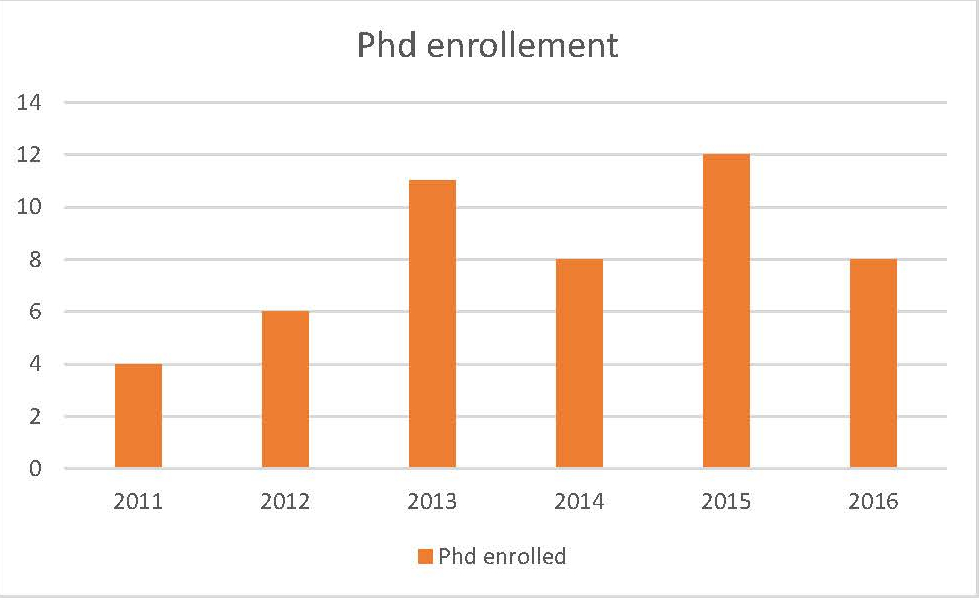
\includegraphics{phdenrollement.jpg}}
  \caption{PhD students enrolled since the last report}\label{phdenrol}
\end{table}

During the same period we undertook a serious effort to increase our capacity to tutor PhD students, by inciting the 
associate professors to defend their ``habilitation à diriger des recherches'' (HDR). Indeed, during these years, 8 among our Associate Professors and CNRS researchers obtained their HDR and at least two more are expected to do so before the end of 2017. This increased tutoring capacity joined to a global effort to attract more PhD students allowed to move our annual recruitement of PhD students to an average of 10 annually. Table \ref{phdenrol} shows the evolution of new PhDs every year (some differences over the years are due to the fact that some PhDs funded by industrial contracts actually start in the middle of the academic year, but are counted sometimes for the following year). Overall we had 46 new PhD students (of which two in management science and one in mathematics, the rest in computer science), with a strong concentration at the last years as a result of our policy.

\begin{table}
  \centering
   \scalebox{0.65}{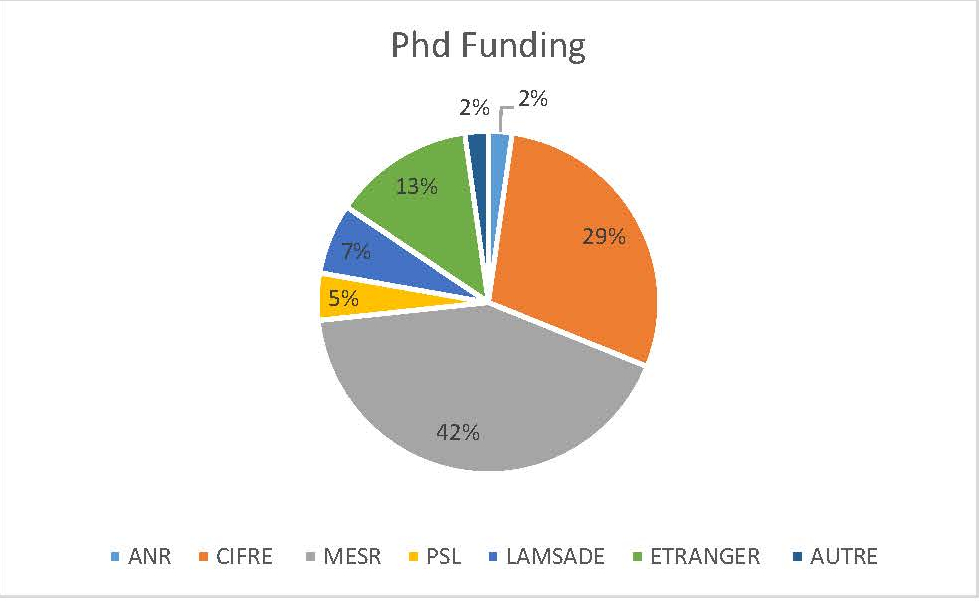
\includegraphics{phdfunding.jpg}}
  \caption{Distribution of PhD funding}\label{phdfund}
\end{table}

These 46 new PhD students have been funded in various ways (there are no non-funded PhD students in the unit). The distribution of the different funding sources can be seen in table \ref{phdfund}. As expected, the largest source remains the scholarships offered by the University through the Doctoral school and more recently by PSL. However, the second more important source are industrial contracts (CIFRE type), this type having become increasingly important during the last two-three years. The third source are PhDs funded by foreign governments, most of the time under co-tutoring agreements (Tunisia, Italy, Burkina Faso, Brazil). It is also worth noting that the LAMSADE has been able to fund 3 PhDs using its own funds (more details in section \ref{Management}). From 2013 on, we introduced a new competitive scheme for the recruitement of PhD students, which is now running in a very satisfactory way, attracting students at an international level (more details in section \ref{policy}).

\begin{table}
  \centering
   \scalebox{0.65}{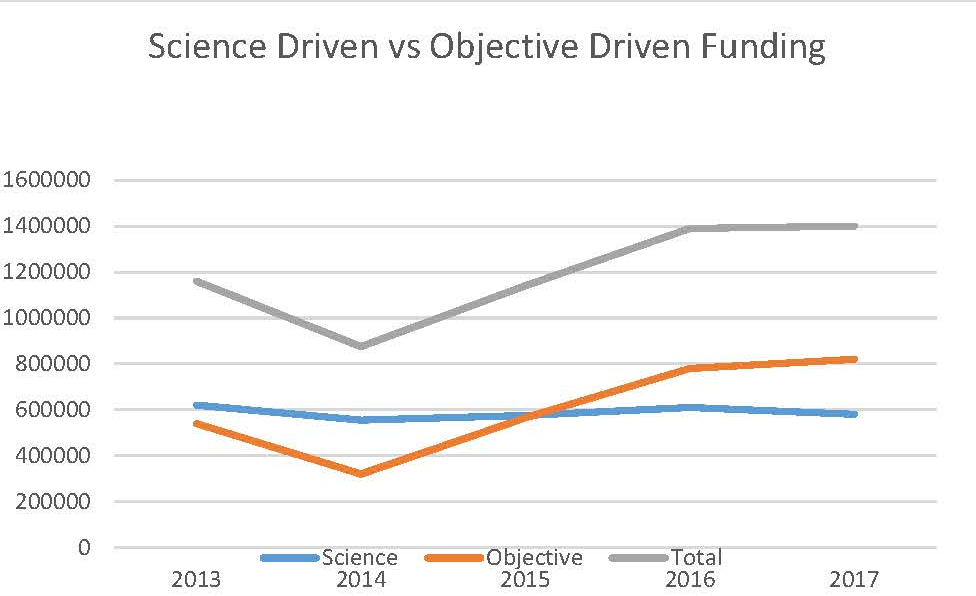
\includegraphics{globalfunding.jpg}}
  \caption{Global funding trends}\label{global}
\end{table}

The LAMSADE has an overall wealthy financial situation. However, in order to explain the global funding diagram presented in table \ref{global}, we need to explain how these figures have been obtained. The starting point has been the expenses of the unit: the everyday life, the research expenses (essentially missions, workshops and hardware) and most important the funding of the PhD students and the post-docs (it should be noted that in these 5 years the LAMSADE occupied 11 post-docs for periods going from 6 months to 2 years). Such expenses have been covered by different sources of income: the general funding coming from the University and the CNRS, the funding obtained competitively through projects (8 ANR projects, 7 PEPS of which 4 JCJC, 6 PSL projects) and the funding obtained directly, but most of the time indirectly, from industrial partners (more than 20 CIFRE contracts plus 5 direct research contracts). In counting the income generated we decided to include the indirect income corresponding to the funding of the PhD students, since this represents a non-negligible effort done by our members in order to secure such funds. The result is a global funding merging the direct funds and indirect ones. These are separated in two categories: the funds obtained on the basis of our scientific reputation and mission (science driven funding) and the ones obtained either through competitive funding or through industrial contracts (objective driven funding). Table \ref{global} shows the evolution of this funding over the last five years. The key figures to bear in mind from this table are: \\
 - the LAMSADE has an overall ``budget'' of approximately \EUR{1.4M}, regularly increasing every year; \\
 - the traditional competitive funding through the ANR has been in large part replaced by the funding from PSL; \\
 - there has been a sharp increase in the last three years of industrial funding essentially through CIFRE contracts (there have been more than 20, most of them recent ones).

As already mentioned, the financial situation of the unit is comfortable at the point to be able to fund on its own resources 3 PhD grants. This, however, should not conceal the fact that a large part of this ``wealthiness'' is obtained through contracts, (relatively) easy to negotiate, but with a limited horizon (for more discussion on this point see section \ref{swot}).

\subsection{Scientific policy}\label{policy}

The missions the LAMSADE, as stated when it was evaluated five years ago, can be summarised as follows:
\begin{itemize}
\item strengthen the international position of the unit as one of the European leaders in Decision Sciences and Technologies;
\item improve the internal life in the laboratory, by increasing participation and commitment;
\item help the early stage researchers to make their way in their careers;
\item make the LAMSADE a nice place to work, to study and to produce good science.
\end{itemize}

In order to strengthen our international recognition, we have been pursuing two main directions. The first one has consisted in strengthening our role of research communities creators and animators. Our positioning in algorithmic decision theory, game theory, computational social choice, parametrised complexity, polyhedral combinatorial optimisation, graph theory among the European leaders is a fact. The second direction has consisted in pursuing both excellence and internationalisation to all of our recrutement actions (PhD students, post-docs or new colleagues). Under such a perspective, we are very proud that we manage to attract people from all over the world to come study with us, to work with us or even to visit us. The LAMSADE is an international crossroad.

However, this policy would have given only partial results if not completed by our clear investment in Data Sciences. The creation of the third team of LAMSADE around this topic, and the recruitement of several new colleagues (6 out of 9) has been a collective effort the whole unit decided to undertake despite the risks and the difficulties such a decision implied. Our investment already starts paying positioning the unit at an international level also in this area.

It has been a deliberated policy to improve and better organise the internal life of the unit: approaching a global size of 100 and with three large teams, and taking into account that more than one third of our scientific staff has been renewed during these years, a clear regulation of our internal life was necessary. This mainly concerned the use of our common resources: funding, PhD scholarships and positions available for temporal recruitements (invited professors or assistant professors) and for permanent ones. The regular meetings of the Council allowed to discuss and establish clear rules for this purpose. It has been a long process, which is not yet achieved since we need to update and revise our rules as we cumulate feedback. It has not been always simple to conduct this process (through misunderstandings, misinterpretations and errors ...), but the rules of our internal life now exist and work.

The LAMSADE continued in these years to pursue its policy aiming at helping the early stage researchers to integrate the scientific life of the unit. For this purpose we have a special fund dedicated to the PhD students and to the colleagues who have just joined us. This allows to cover scientific missions otherwise impossible to undertake. Further on we decided, when the PhD grants are distributed, to give the priority to proposals coming from our ``young'' associate professors in order to give the opportunity to start directing a PhD student (this being one of our fundamental missions).

The structure of the unit has already been presented in Section \ref{presentation} and in Table \ref{organisation-en}. The three teams of the unit are aimed to conduct essentially research animation (seminars, invitations etc.) and to federate colleagues sharing a broad scientific area within the LAMSADE area. The ten projects instead are aimed to conduct long-term research activities on a given subject, which we expect to last for a sufficiently long period (such as 10 years). The projects are aimed to raise their own resources. These projects do not necessarily ``belong'' to a team. Actually five of them intersect two or even three of the teams both in terms of research subjects, but also in terms of people involved (it is the case that people from several teams contribute to the scientific life of the projects).

In choosing our research priorities, we consider the following guidelines: \\
 - allow the LAMSADE members to pursue their own individual research interests; \\
 - provide a scientific identity to the unit justifiable and compatible with the identity and policy of Dauphine (and more recently PSL); \\
 - fulfill the high standards in terms of quality and management required by the CNRS; \\
 - maintain at least 10 years of scientific advantage (in terms of knowledge) with respect to the demand of the society; \\
 - be able to respond positively to the challenges our society (France, Europe, World) present us.

As a CNRS research unit, our fundamental mission is to conduct fundamental research. However, we need to consider two constraints in pursuing this mission. The first derives from the fact that funding for fundamental research is decreasing. Or to be more precise: funding for science-driven research is decreasing. We define science-driven research as activities guided by our knowledge, training, experience and intuition as researchers: research which is not expected to deliver a precise result, but to advance knowledge and attack challenges which most of the people and the organisations around us ignore or do not consider actual. However, it is this type of research that delivers the results and the knowledge in order to handle the problems our societies will face 10 or more years from now. Given the present situation, where this type of research is generally undervalued, we decided to dedicate part of resources in funding ``science-driven'' PhD grants (besides the ones offered by the University). We have been able to fund 3 such grants. The second constraint is related to the specific nature of our research in decision sciences and technologies. Our objective is to improve how people (and automatic devices) decide as well as how analysts help people (and automatic devices) to decide. Decision making and aiding decision making are essentially empirical activities and the inputs for innovation in our field have always been offered by real life. Under such a perspective it is essential for a unit like the LAMSADE to keep a constant contact with the demand for decision support the society around us presents. For this purpose we consider the societal challenges around us as research challenges and we dedicate part of our research being implied in real cases of decision aiding (this being any among models, algorithms, data structures, services etc.). The result of these two constraints is that the LAMSADE has a policy of wise equilibrium between science-driven and objective-driven (reply to a precise challenge) research.

In order to conclude our policy presentation, we may mention that it has always been a priority trying to make the LAMSADE a nice place to work and study. Besides enabling our members to conduct their research with as less hassle as possible we try to promote cooperation, mutual respect and understanding, equal opportunities and a lively environment for discussion and exchange of ideas. The fact that we receive every year a very high number of foreign visitors contributes very much in this direction. However, we may also mention that we also try to promote an idea of research as ``having fun'', since this is an essential component for the creativity research requires. We do serious research, but we are very proud not to be always serious!

\section{Production}\label{secproduction}

A global overview of the scientific production of the LAMSADE can be seen on Table \ref{production}. In this table we counted only peer reviewed journals, selective international conferences, books, chapters in books and edited proceedings and volumes. Quantitatively, the unit has a practically constant production of a good level: considering an average presence of 50 permanent scientists within the LAMSADE during the period considered we get an average production of 3 publications per scientist per year.
\begin{table}
  \centering
   \scalebox{0.65}{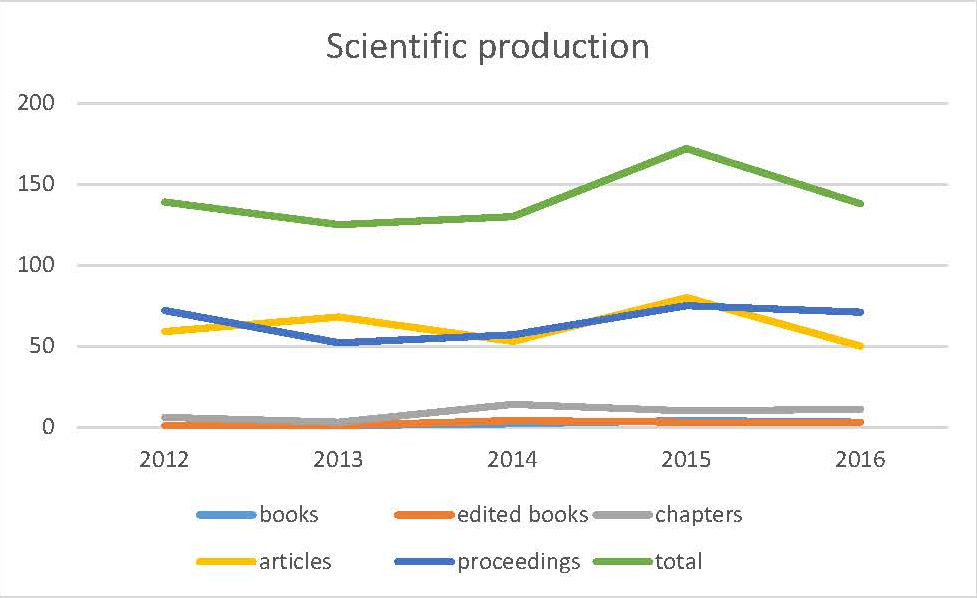
\includegraphics{production.jpg}}
  \caption{Global scientific production of the LAMSADE}\label{production}
\end{table}

To this result we may add the fact that the LAMSADE members are present in the editorial board of more than 30 international journals (one editor in chief) mainly in the area of Operational Research and Decision Analysis and in an uncountable number of scientific committees of international conferences including some among the more prestigious ones. The members of the LAMSADE have been invited to give talks/lectures/tutorials to more than 100 conferences and workshops around the world (not counting the personal invitations for seminars and visits). Let us also mention that during these years the LAMSADE received the visit of more than 80 foreign colleagues from more than 35 different countries for approximately 100 months of invited professor. Last, but not least during this period there have been 36 PhD defenses (the average duration of a PhD thesis being 3,9 years) and 8 HDR ones (for a discussion about the job destination of the former PhD students the reader can see Section \ref{swot} and Table \ref{phdjobs}).

However, these results do not reveal the qualitative evolution of our scientific production. While we kept a constant quantitative production the quality of our papers sharply increased. Journals such as Mathematical Programming, INFORMS Journal of Computing, Artificial Intelligence or JAIR now regularly publish our results, while top tear conferences such as IJCAI, AAAI, AAMAS, ICALP, ESA, EDBT, WWW are now regularly visited by our researchers presenting their results.

A detailed presentation of the scientific achievements of the three teams can be seen in \cref{team1,team2,team3}. In the following, however, we give a rapid outlook of the major scientific achievements of the LAMSADE in the last 5 years.

\vspace{5mm}

1. The axiomatic characterisation of bibliometric indices as well as the axiomatisation of preference aggregation procedures based on the concordance/non discordance principle (\cite{Bouyssou2015A-634565}). \\
2. The GRAVE algorithm, designed as a generalisation of the well known RAVE algorithm which greatly improves its performance in many games; see \cite{Cazenave2015Generalized-1222829}). \\
3. The Handbook on Computational Social Choice (presented in 2016): in this book which is now a landmark of this research topic, one of the editors is a LAMSADE members, 3 out of the 19 chapters of the book are co-authored by members of the LAMSADE, while 8 others by invited professors of our unit (sometimes during their stay at LAMSADE; see \cite{HBCOMSOC2016}). \\
4. Two nice real world applications of our research: the first concerning the use of MCDA methods in order to evaluate different layouts of the new rail line from Paris to Normandie and the second concerning the use of inverse Banzhaf indexes in order to find the proportion of seats for each Institution within the Academic Council of PSL (the actual distribution of seats is the one our method suggested). \\
5. In the area of Complexity and Approximation two results can be considered as outstanding: \cite{DBLP:journals/algorithmica/BonnetE0P15} proposes a formal framework for super-polynomial approximation (mainly sub-exponential and parameterized) and provides inapproximability results for paradigmatic problems (as maximum clique, dominating set, etc.) in this framework, while \cite{Karpinski2015New-1298222} tightens the known inapproximability bounds for the Metric Travelling Salesman Problem. \\
6. Two breakthrough contributions which we recently contributed in Mathematical Programming. In \cite{DBLP:journals/mp/AissiMMQ15} the multiobjective and parametric versions of the global minimum cut problem in undirected graphs and bounded-rank hypergraphs with multiple edge cost functions are studied. They proved that for a fixed number of edge cost functions, the total number of supported non-dominated cuts is bounded by a polynomial in the numbers of nodes and edges. In \cite{Cornaz2014Chromatic-623556} the quality of Lov\'asz theta function, as a bound for colouring, is improved using graph theoretical tools. \\
7. A main contribution in the field ``Multiobjective combinatorial optimization'' is the introduction of the concept of search region~\cite{Klamroth2015On-634730,Dachert2017Efficient-1250848} which enables the design of efficient algorithms generating exactly or approximately the non-dominated set.  Another original stream of research deals with the generation of the preferred solutions in the sense of aggregation models such as OWA~\cite{Galand2012Exact-610325}, Choquet~\cite{DBLP:conf/ijcai/GalandLP13}, Lorenz~\cite{Galand2015Exact-1052488} or a partially defined weighted sum~\cite{Kaddani2017Weighted-1232001}. \\
8. A major advance in data integration has been done by showing that the cost of ensuring good quality of integration can be reduced dramatically using a small number of feedback instances solicited from end users \cite{Belhajjame2013Incrementally-904545,DBLP:journals/dpd/BelhajjamePHF15}. In the context of BigData, the PAQuery systems has been proposed \cite{DBLP:conf/sigmod/Camacho-RodriguezCM14, DBLP:journals/tkde/Camacho-Rodriguez15}, providing the first formal specification and implementation of a powerful compilation technique from the XQuery query language to PACT, a powerful extension of MapReduce. \\
9. Within the context of a collaboration with Google (Google Brain at NYC and Google Research at Palo Alto), Nvidia, Columbia University, Courant Institute, and CEA List, we proposed in~\cite{Bojarski2017Structured-1259771} a new framework for speeding up several machine learning algorithms (e.g. kernel approximations, deep learning, LSH, etc.) with almost no loss of accuracy. In the context of Computer Games, we continued our seminal works on Monte Carlo Tree Search (MCTS) and proposed significant improvements to the architecture of the deep neural networks of AlphaGo~\cite{cazenave2017residual}. In the context of generalization of regret minimization to the Blackwell approachability setup,~\cite{FLP2016} shows that unlike in standard online learning literature, the necessary or sufficient conditions for the anytime version of this problem are drastically different than those for the fixed horizon. \\
10. Based on our experience on process mining and matching, we participated in writing a monograph (published by Springer) \cite{DBLP:books/sp/BeheshtiBSGMBGR16} that surveyed approaches and tools for process analytics (co-authored with experts in the field from UNSW Australia, IBM Almaden Research Center,... ). Concerning services, we have proposed several solutions and a complete analysis of complexity and models for service discovery, composition and execution problems, taking into account non-functional properties  \cite{GMMM17, AngaritaArocha2016Modeling-1159056}. In a seminal work~\cite{Abu-Khzam2015On-1017005}, we have a comprehensive study and prove of the exact complexity of the service selection problem by taking into account QoS criteria for single and multi-criteria instances.\\
11. An important breakthrough has been the establishment of a new interdisciplinary research subject: policy analytics (\cite{Belton2013Policy-624015}) aiming at improving decision aiding in designing implementing and evaluating public policies. A new national (\url{www.gdr3720.fr}) and international scientific community are now under construction.
\vspace{5mm}

Overall the LAMSADE is proud of the work accomplished during these years. However, there are a number of highlights for which we are particularly proud and we may illustrate in the following as examples of our achievements.

1. In 2014 the LAMSADE celebrated 40 years of activities (it has been created in 1974). We organised during the year 4 lectures involving Google, Frédérique Ségond, Christos Papadimitriou and Hervé Moulin, all of which had a great success. These lectures contributed significantly to the scientific reputation of the unit (both within our strict environment and beyond it). This visibility has been completed by the delivery of three Doctor Honoris Causa to three outstanding colleagues: Fred Roberts, Christos Papadimitriou and Claudia Bauzer Medeiros. \\
2. In 2015 we received 4 CNRS researchers who are not Computer Scientists. It has been a massive sign of trust from the CNRS and at the same time a huge challenge for the LAMSADE: become able to integrate different disciplines under the Decision Sciences and Technologies perspective. We are proud to see this challenge turning into a success (completing other interdisciplinary initiatives such as the Master in Peace Studies). \\
3. In 2016 the LAMSADE undertook a large restructuring ending with the establishment of the Data Sciences team and the appearance of new projets enabling the appropriate visibility of cross-laboratory research subjects such as social choice, game theory or machine learning. It has been the end of a process started in 2012 when the recrutement policy of the unit has been first discussed and is now continuing as a challenge for the whole LAMSADE for the future. \\
4. In 2016 Bernard Roy received the EURO Distinguished Service Medal strengthening the already well known reputation of the LAMSADE in the domain of Operational Research and Decision Analysis (it should be noted that the LAMSADE is the only OR laboratory in Europe who has an EURO Gold Medal, 2 former presidents of EURO and now the EDS Medal). The same year Stéphane Airiau coauthored the paper which won the ``Best Paper Award'' at the prestigious AAMAS conference (\cite{Airiau2016Rationalisation-1088325}). \\
5. In 2017 we received a very prestigious recognition of our efforts. Jérôme Lang and Eunjung Kim received the CNRS silver medal and bronze medal (respectively) in Computer Science. It is the first time that the same research unit receives the same year two such distinctions. It should be noted that during the period under consideration Cristina Bazgan and Vangelis Paschos were recipients of two IUF grants (junior and senior respectively). \\
6. During this period we increased our efforts in order to enhance and improve our outreach both for specialised audiences (other than computer science) and the general public. Despite our natural aversion for too much advertising we have been able to comunicate on several ``hot subjects'' including Artificial Intelligence and Machine Learning (thanks to our colleague Tristan Cazenave who now regularly appears on the media for his expertise in AI). However, the single project for which we are very proud is the video we produced in order to celebrate our 40 years. We have been asked to prepare an institutional advertisement of our activities and we ended preparing an unconventional story about who we are and what we do. We are still able to have fun and to make a joke of ourselves in this laboratory.
%2. Scientific production and activities (for the unit, and next for each team and/or theme of the unit)
%Sections 2-5 will be filled first for the whole unit, and then for each team and/or theme of the unit.
%Scientific output
%The unit (or the team /theme) will give a global overview of the scientific outputs of the current contract.
%Quantitative data
%Quantitative data on the whole production and activities of the unit or team/theme are to be given in the Excel file “Données du contrat en cours”, Table 5, “Scientific production and activities”.
%Selected production and research activities
%Please provide a selection of the unit or team/theme scientific production and activities (in appendice 4, see page 4). Concerning the scientific production (paragraphs I, II and II), the list has to be limited to the most significant 20%.
%The complete list of production and activities of the unit or team/theme needs to be provided (for example on a website) to the committee upon request.
%Highlights
%Here, the unit or team/theme will briefly discuss a restricted number of highlights concerning any of items of the scientific production and research activities.
%Please adjust the number of highlights to the size of the unit or team/theme.

\section{Management}\label{Management}

The management structure of the LAMSADE is summarized on Table \ref{organigramme}. As usual happens there is a director (and a vice-director) a Council of the unit, an administrative team and three teams leaded by their respective coordinators.

\begin{table}
  \centering
   \rotatebox{-90}{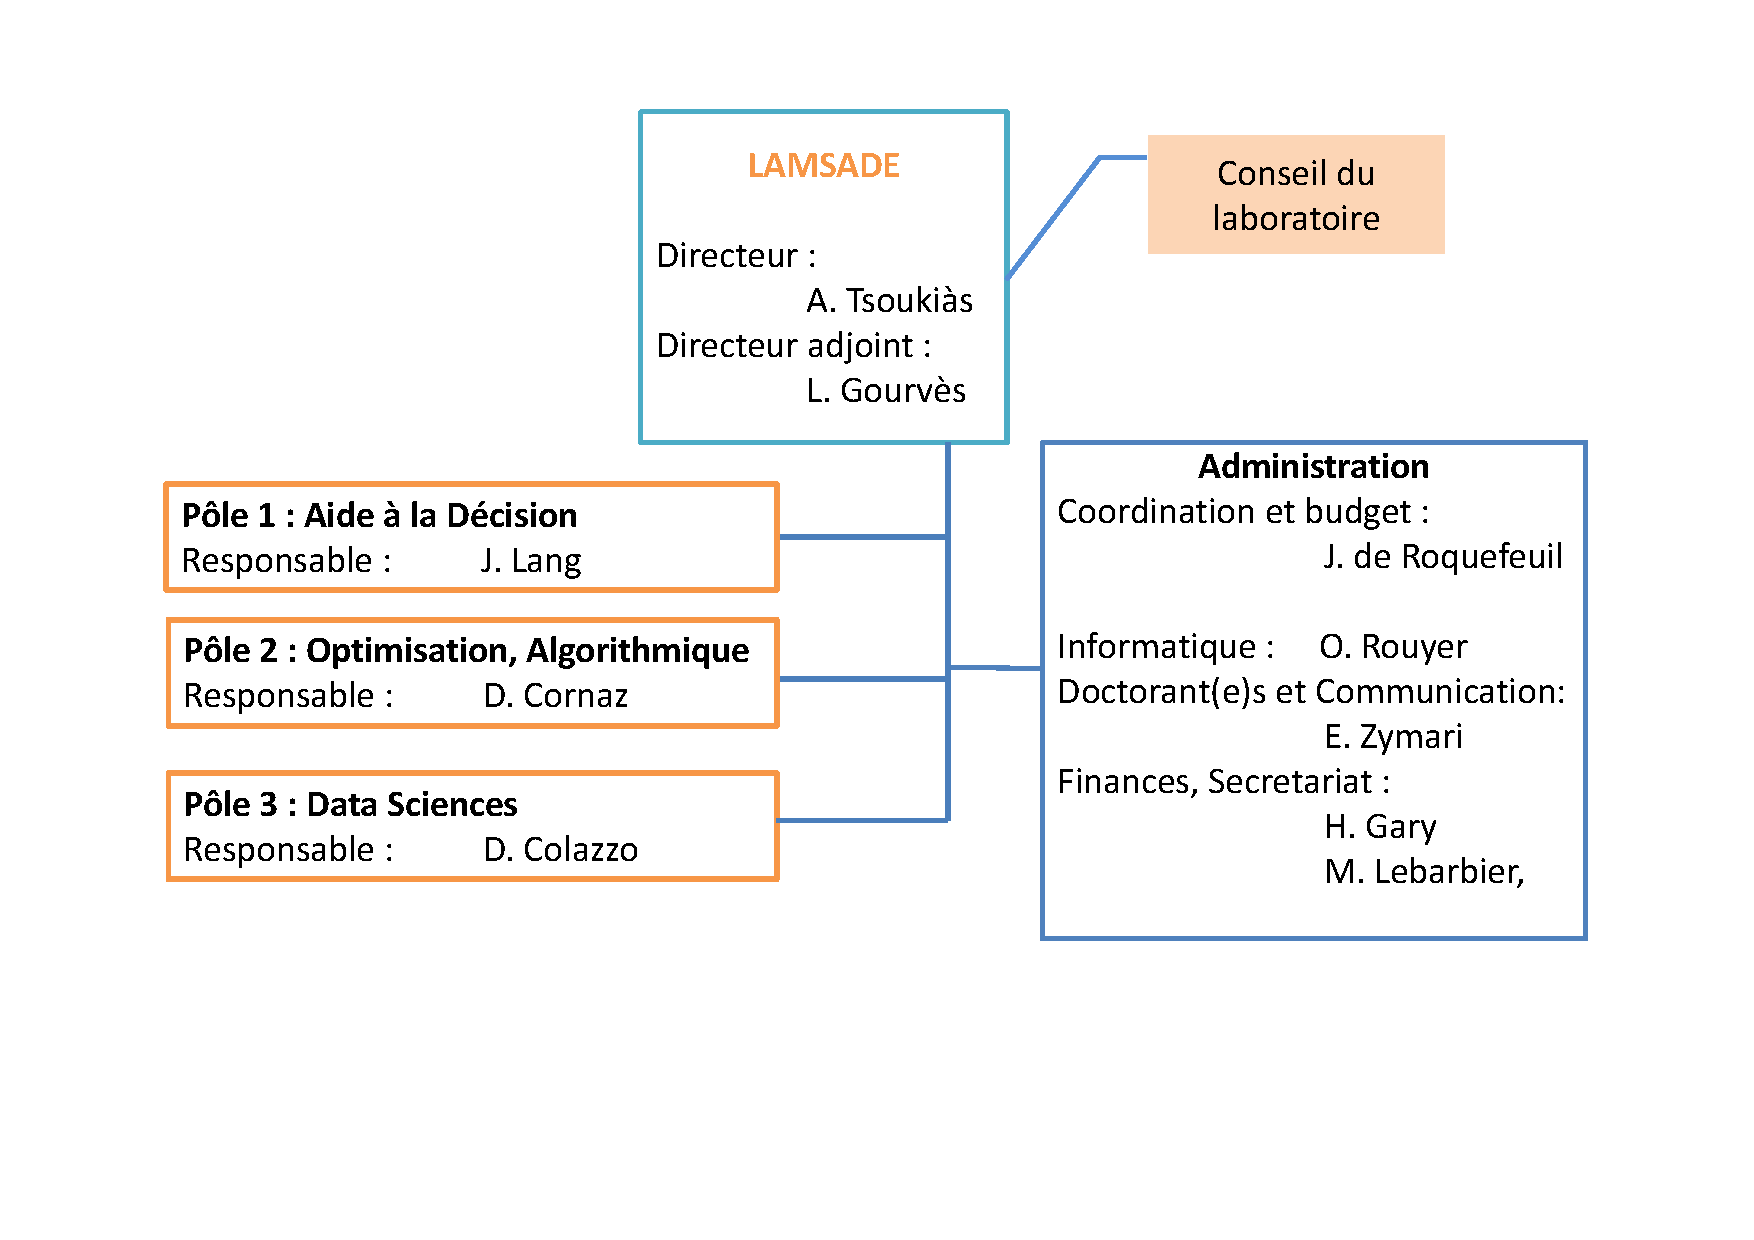
\includegraphics[height=\textwidth]{organigramme.pdf}}
  \caption{LAMSADE management structure}\label{organigramme}
\end{table}

The management of a research unit of the size of LAMSADE is relatively simple. First of all there are two major regular collective moments in the life of the unit: \\
 - the LAMSADE day, occurring usually at the beginning of spring, dedicated to scientific discussion, the presentation of the new colleagues, of new research projects etc.; a speed presentation (180 sec.) of the second year PhD students also takes place; \\
 - the general assembly (GA) of LAMSADE, occurring the third Tuesday of June, where the policy of the unit is discussed for at least one critical issue (training, scientific strategy etc.).

The organisation of the LAMSADE days started in 2012 and evolved during these years to the present format (stable since 2016) which seems to satisfy most of the members. It should be noted that in 2014 we did not organise the LAMSADE days due to the celebrations for the 40 years of the unit. The two main subjects discussed in the GA of the unit have been the creation of the Data Sciences team and the innovation of our training offer in Computer Science (on that last topic there have also been a couple of exceptional GAs).

The life of the unit is essentially organised by the 3 teams and the 10 projects. However, as far as management is concerned, the 3 teams regularly meet in order to discuss at a decentralised level topics related with the policy of the unit, while this is not the case of the projects. The teams mission is to animate discussions (seminars and policy issues). The teams also have a budget (\EUR{15K} annually coming from the general budget of the unit) which is expected to support missions and other scientific animation activities. On the other side the projects (5 of which are transversal to the teams; see Table \ref{organisation-en}) are expected to conduct research (most of the times through PhDs and Post-Docs), to organise scientific events and to contribute to the global fund raising of the unit. Under such a perspective the projects do not receive a regular budget from the general one (although may occasionally ask for some support), but they compete for a critical resource which are the PhD scholarships.

The unit is managed by the director (and the vice-director) assisted by the administrative staff in interaction with the Council of the unit. The latter is the typical consultative structure of all CNRS units: it is expected to be consulted on all critical issues of the unit's life. It is composed by 15 members (plus the co-director of MIDO and the administration responsible who are permanently invited): \\
 - the director and vice-director; \\
 - 9 elected members (7 among the scientific staff, 1 among the administrative staff and 1 among the PhD students); \\
 - 4 appointed by the director. \\
It meets 8 times during the year (always on Tuesdays at noon) on rolling dates which are now becoming stable. Besides discussing regular topics (budget, recrutements etc.) it also has a special mission: identifying every year the subjects for which we look for PhD candidates, organise the hearings of the candidates and prepare a ranking which is submitted to the Doctoral School. \\
For most of the everyday issues the direction and the staff are sufficient. Occasionally there are cases where an enlarged version of the direction meets including the three team leaders.

Parallel to the Council there is the CCR (a Representative Consulting Committee) required by the statutes of Dauphine and concerned by the hiring of scientific staff (in the case of LAMSADE in Computer Science). This Committee is led by the director of the LAMSADE, it is composed by 20 members (10 full professors or research directors and 10 associate professors or researchers), 16 of which are elected, 3 being appointed by the director, the director being also a member. This committee meets 3 times during the year: \\
 - in late autumn in order to fix the essential lines of any recrutement profile and to identify the person in charge of the selection committee (any long term policy issues are also discussed in this meeting); \\
 - in late winter in order to approve the profile of any recrutement and the selection committee; \\
 - in early summer in order to rank the applications for invited professors and the applications for assistant (not permanent) professors.

As already mentioned the LAMSADE is one among the few research units in Computer Science with more than one third of its permanent scientific staff being women. We are very proud of this and we actively pursue ways aiming to maintain this situation with particular emphasis to all recruiting opportunities.

\section{SWOT}\label{swot}

There are multiple strengths at the LAMSADE. The unit has a well established identity (Decision Sciences and Technologies) which spans from our traditional subjects (Operations Research, Decision Theory, Algorithms, Artificial Intelligence) to the more recently added ones (Machine Learning, Database Management etc.), thus covering the whole range of Computer Science and Decision Sciences. We have a regular administration, clear rules for the distribution of all critical resources and a wealthy financial situation. We produce very good science and our international reputation has never been stronger. We have taken up an interdisciplinary challenge, which for the time being works fine with respect to all the disciplines with which we cooperate; more importantly, we attract researchers from other disciplines to come and work with us. We have also taken up the challenge to become more international, and this has also been a success. We attract colleagues from all over the world as well as PhD candidates. There is, however, one single strength for which we are proud and for which we consider the LAMSADE as unique: the fact to have created and contributed to create several international research communities. We do not only anticipate the scientific challenges (as any fundamental research unit should do), but we create the communities who will take care of them. Decision Sciences and Technologies is a niche domain requiring strong networking activities: the LAMSADE is at the unit of these networks.

There are also clear weaknesses. Undoubtedly the establishment of the new team has been unevenly perceived within the laboratory as there are obvious differences among the three teams. It is certainly unfair to compare a team established since the creation of the LAMSADE and one created only since 18 months. Besides and on the long run such differences are not expected to stand (the Data Sciences colleagues are doing an excellent work which will not take a long time to show the results), but for the time being these exist and could create frictions within the unit. To some extent, this is related to the low visibility our research projects presently have, an issue which needs to become a priority in the near future. However, there are two major weaknesses which need to be considered in the very near future. The first concerns the capacity of the unit to secure long term funding for fundamental research. The present financial wealthiness should not conceal the fact that this is secured thanks to short term objective driven contracts, easy to obtain, but far from representing the ambition that a unit like the LAMSADE should have. The second concerns the attractiveness of Computer Science training at Université Paris-Dauphine. Although this is an issue which concerns more the Department of Mathematics and Computer Science (MIDO) it is clear that the LAMSADE, representing de facto the whole Computer Science community of the University is directly concerned. The fact is that the attractiveness of Computer Science is unevenly distributed among the various training programs and we are yet missing a situation where our scientific reputation could be transformed to attraction for prospective students.

Which are the opportunities offered by the environment where the LAMSADE evolves? Under a contingent point of view this is a time where the knowledge owned by the unit is highly demanded by the society. The investments we did several years ago specialising the unit in areas at that time ``of little interest'' turned to be today a big advantage. At the time where the government considers for instance that the domain of Artificial Intelligence should become a national priority, we are proud to know that we are among the leaders in this area. The same applies to other domains such as Data Sciences, Analytics or the social responsibility of algorithms. There is a huge demand out there in the real world and we can catch it. On a longer run the fact that we showed our ability to conduct interdisciplinary research and to create new areas of scientific investigation at the edge of several disciplines corresponds to a demand of increasing scientific contamination and for new frontiers. We know we can handle such challenges. Last, but not least, the increasing internationalisation of training among European countries and the increasing mobility of students across Europe represents a huge opportunity for innovating our training programs and diversify our training offer policy with big potential positive impacts.

\begin{table}
  \centering
   \scalebox{0.65}{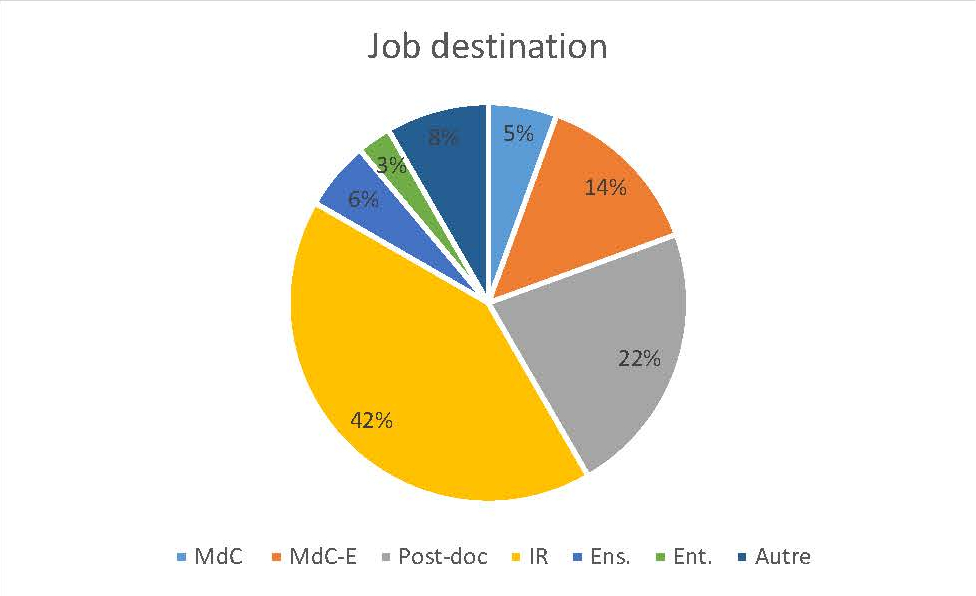
\includegraphics{phdjobs.jpg}}
  \caption{Job destination of PhDs}\label{phdjobs}
\end{table}

Certainly, there is a number of threats we need to consider. Some of them are completely out of our control: both at a national and at a European level there is a persistent policy of downsizing the research infrastructure (particularly the manpower both in research/training and in administration/support) and the science driven funding. At a certain point this will have dramatic effects. Our young colleagues have increasingly less opportunities to pursue their career (unless they turn to the private sector where there are certainly excellent offers from giants of the Computer Science and Decision Sciences business; it has been the case for one of our associate professors and for brilliant young PhDs who finally decided for this option). It is a trend confirmed by Table \ref{phdjobs}: the vast majority of our PhD students is in the private sector. Our research also is suffering: when the prior probabilities of being funded through a competitive call start falling beyond 20\% (sometimes less than 10\% or even less than 5\% ...) the expected utility of introducing an application is negative. If, as presently happens, obtaining an industrial contract is relatively easy, our researchers increasingly turn their eyes to these relatively ``short term'' objective driven research. But on the long run this is not sustainable: the replacement of ideas used with new ones is too slow and soon or later we will find ourselves with no new ideas ... A relatively more contingent and local threat is represented by the relatively modest size of Computer Science (as a discipline) within PSL. PSL de facto represents an important actor (for institutional reasons, for the volume of resources they manage, for the international impact it has), but Computer Science is a marginal subject and discipline within it. Although the two principal research units in Computer Science within PSL (the LAMSADE and the DIENS) have a large international reputation and recognition, their quantitative size is too small with respect to other disciplines and research fields. This requires an accurate strategy of scientific and interdisciplinary alliances, but this is a topic for our strategy section.

\section{Strategy}\label{strategy}

To a large extent, the strategy of the LAMSADE for the next five years derives from our SWOT analysis and the elements we highlighted while presenting the activity report of the unit. We may summarise our priorities in 5 specific areas where we need to concentrate our efforts during the next years: International Visibility, Computer Science Training, Dauphine and PSL, our structure and our funding, our human resources.

\begin{enumerate}
  \item \textbf{International Visibility}. The LAMSADE already has a strong international reputation. As already mentioned we do not only produce good science which is internationally recognised, but we also took several times the initiative to co-create and co-conduct national and international scientific communities. That said, it needs to be understood that, in several fields of the area of Decision Sciences and Technologies, international leadership is now expressed by large global private companies whose R\&D departments largely dominate in terms of size and resources most if not all university research units and departments. Under such a perspective a direct competition on mainstream subjects risks to be counter-productive and not sustainable on a long term. If the LAMSADE wants to be considered as one of the leading European units in this area (Decision Sciences and Technologies) it needs to focus on subjects which either escape the short to medium perspective of this type of competitors or correspond to societal needs and challenges underestimated and thus more or less ignored. In other terms, on the one hand we need to focus ever more now on our fundamental research subjects anticipating the scientific challenges at an horizon of 10-15 years (new optimisation methods, new schemes of algorithmic complexity, new models for learning etc.) and on the other hand we need to produce convincing results as far as critical societal problems are concerned (citizen participation, policy design, society polarisation, homeland security, just to mention a few of these).

      On these subjects and with such objectives we need to attract to the LAMSADE people from all over the world (PhD students, post-docs and scientific staff) willing to participate to our scientific adventure. At the same time we need to strengthen our presence and leadership to all communities where we are involved and foresee the creation of new ones (such as the one concerning the social responsibility of algorithms). We also need to take advantage of our interdisciplinary perspective in order to maintain an innovative perspective to the challenges in front of us.
  \item \textbf{Attractiveness of computer science training}. Despite the LAMSADE not being directly involved with the design of the training activities (these being delegated to the Mathematics and Computer Science Department: MIDO) it is obvious that any initiative concerning the training in computer science has a direct impact to the life of the LAMSADE. Having attractive computer science training programs means having good students to work with, a stimulating environment for consolidating knowledge, improving international visibility and attractiveness (after all we try to attract colleagues who are going to teach most of the times), expanding the outreach of our work.

      The subject has been discussed several times in the recent years in dedicated meetings of the computer scientists of Dauphine (which more or less corresponds to the members of the LAMSADE). There is an uneven attractiveness of the different training programs, there is an uneven visibility of these, but what is perhaps most important is that we do not present a global vision of what means for a young student to be trained in Computer Science at Dauphine. The result is that we still miss a global vertical program in Computer Science.

      Our aim is, in cooperation with our colleagues in CEREMADE and more generally MIDO, to design a more comprehensive and readable program in computer science (lasting 5 years, under different formats) including an horizontal training program in mathematics and computer science at the bachelor level. This is not the place where these ideas ought to be developed; we want to affirm our commitment for an innovative and attractive program in computer science (and in mathematics) at Dauphine.

      Besides this commitment, we need to quantify and improve the way through which computer science is taught in training programs which are not in computer science (management, economics etc.). Last, but not least, it is important to maintain our commitment to the interdisciplinary program of Peace Studies which has been created under our initiative and today presents a big success for the whole University and the PSL.
  \item \textbf{Dauphine and PSL}. When the previous evaluation exercice of the LAMSADE took place PSL was more a project than a reality. Today PSL is a strong reality and despite the problems all new endeavours have, we are expecting it to become a hard constraint to our everyday life as a research laboratory. We already mentioned that PSL can be seen both as an opportunity and as a threat. An opportunity because of the resources it mobilises, the international visibility that can add and the challenges it represents. A threat because of the relatively modest quantitative presence of computer sciences (and even less Decision Sciences and Technologies) within it. The practical risk is to see once again the computer science considered as a service and not as a discipline by itself. To some extent, this is an experience we had the early years within Dauphine, where Computer Science was relatively modest. There are three actions the LAMSADE can and has to undertake in order to strengthen its position and at the same time strengthen Dauphine and PSL as Global Higher Education and Research Institutions. \\
      1. The first consists in strengthening the relations and cooperation with the computer scientists within PSL (mainly the DIENS which is the other strong reality in computer science within PSL). We already have a number of joint projects, but regrettably there has been no coordination among the two units and this needs to be improved: we expect the discussions about the computer science training within PSL and the existing positive experiences may help in that direction. \\
      2. The second consists in further developing our interdisciplinary potential. Several among our research projects (Social Choice and Games, Policy Analytics) and training initiatives (Peace Studies) have a strong interdisciplinary nature which addresses forces beyond the computer scientists creating alliances (in Economics at ENS, in Management in École des Mines, in Social Sciences at EHESS) through which increase the awareness of the importance to have a strong component in Decision Sciences and Technologies within the PSL. \\
      3. The third consists in using our enormous international network in order to promote initiatives that could help on the one side the international recognition of PSL and on the other side to promote our research. Under such a perspective our recent initiative to establish a UMI implying PSL, CNRS and ANU is a typical action in this direction.
  \item \textbf{Structure and Funding}. The LAMSADE has now a stable structure which we do not expect to put under discussion in the following years. That said, it is natural to expect that the 10 scientific projets, through which we essentially produce our research, may look for more visibility, gain an increased autonomy and turn to be the essential units of the unit.

      On the one hand, this structure allows the members of the LAMSADE to participate to more than one project enabling them to pursue their scientific interests in a much more flexible way. On the other hand, this is a much more agile structure allowing to mobilise and attract ressources mainly through competitive funding. It also allows to adapt much better to the demands originating from societal challenges we may want to follow.

      A critical priority for the LAMSADE will be to secure long term funding for the research conducted within it. We already mentioned that the present situation, although allowing a relative wealthiness, should be carefully monitored as far as the impact of short term contracts has on our research priorities and subjects. The unit should push the many brilliant researchers within it to apply for ERC grants, H2020 projets and through other long term funding schemes. A target for raising \EUR{3-5M} in the following 5 years is feasible and needs to be pursued appropriately.
  \item \textbf{Human Resources}. The LAMSADE is first of all a place where approximately 100 people work together. This living experience needs to be positive for the ones who participate. This concerns the permanent scientific staff, the PhD students, the post-docs and the technical staff.

      Securing such a positive experience requires first of all fulfilling some simple conditions: some we already do (clear and simple rules in order to distribute common resources, scientific animation, international exposure), some other we still unfortunately miss (physical space, both individual and collective), but we hope to be able to secure in the future. In any case it remains among our top priorities.

      However, we also need to be able to take care of the personal aspirations of our colleagues mainly as far as the ``young'' ones are concerned. We cannot certainly take care individually, but we can guarantee that the LAMSADE offers the conditions under which each individual can develop his own personal plan.  Once again we already have a policy which promotes and helps the ``younger'' among us, but we need to go further on distributing and redistributing all collective charges, promoting long life training and dedicated sabbaticals (including the technical and administrative staff), promoting a risk-taking scientific attitude etc. An objective here is to be able to fix an average maximum time of remaining at the same level as well as target situations of the type: within X years Y\% of our younger scientists have their HDR and are de facto able to start looking for a promotion.

      Overall the LAMSADE needs to remain a place where the members have to spend nice days ... where it should be still possible to have fun ... a place to regret leaving when being promoted.
\end{enumerate}
